\chapter{Motions}
\label{chap:Motions}
\begin{figure}[H]
    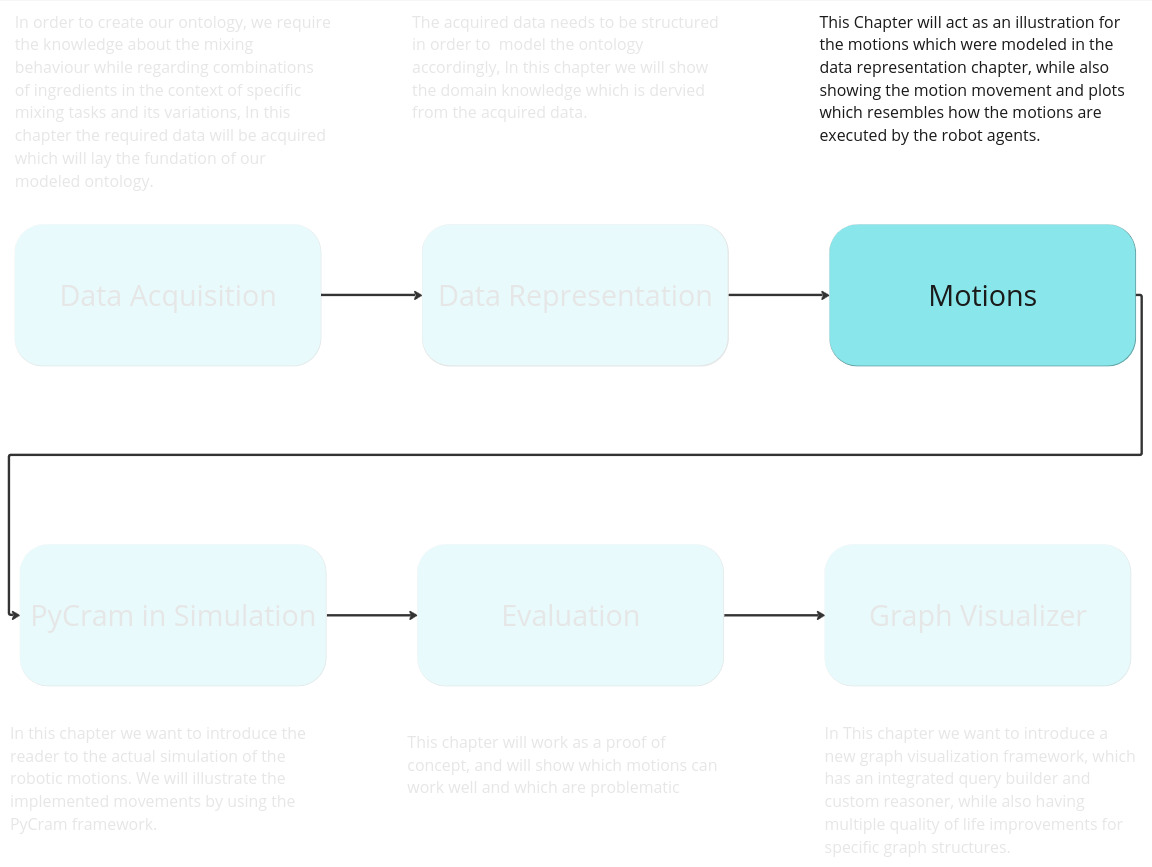
\includegraphics[scale=0.3]{Graphics/overview_3.jpg}
\end{figure}
In this chapter we'll describe on an abstract level how the motions are implemented in pycram2.
To simplify the implementation of motions, we hold the following assumptions about the motions which are performed on containers.
Firstly we assume, the container is symmetric in the x,y direction. We don't consider the descent of the container, we keep the height for the tool
constant over the performed motion. We don't have collision detection.

\section{Circular Motion}
The circular motion is generated on a circular plane. 
By having a center coordinate = $(x,y)$, which is the center coordinate of 
the container to execute the Circular Motion, we generate a set of coordinates
with the following functions: 

\[x = centerX + radius * cos(radian)\]
\[y = centerY + radius * sin(radian)\]

We retrieve the respective radians using the following function:

\[radian = angle * \frac{\pi}{180}\]

Generating a sequence of points lying inside a circle is accomplished by generating a sequence of angles starting from 0 to 360 degrees, 
converting them into radians, and using formulas to compute the circular coordinates.

\begin{figure}[H]
    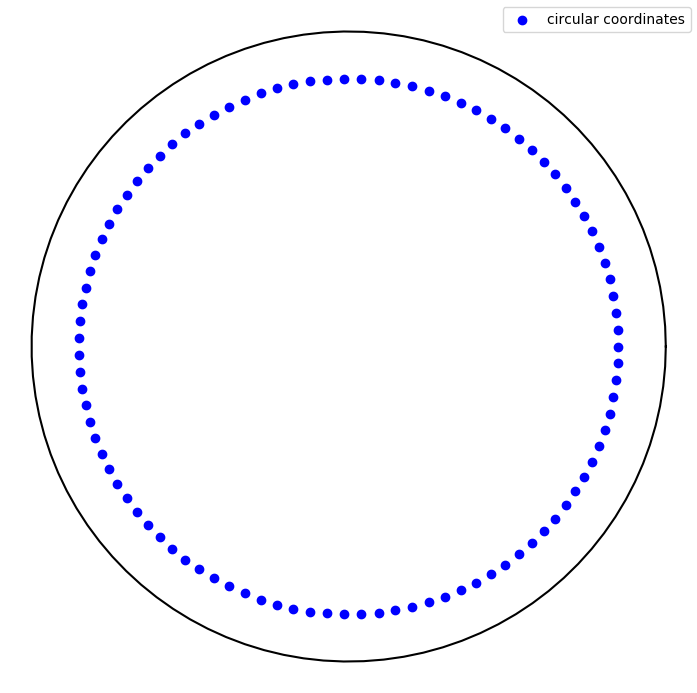
\includegraphics[scale=0.35]{Graphics/motions/circular_motion.png}
    \centering
    \label{fig:circularMotion}
    \caption{Top Down View - Circular Motion}
\end{figure}

\section{Folding Motion}
The folding motion is not a circular motion but rather a linear motion. In its current implementation, the motion is a singular line having where one endpoint is on the edge of the container
the other is center of the container. While the motion in itself is a straight line going through the container, the motion is executed by traversing from one end of the container to the center,
and then repeating the motion flipped - from center to one of the end, which creates a folding effect.
This line partially covers the whole container, therefore the direction has to be realigned in order to mix different sections of the container.

By constructing a 2D rotation matrix for some angle, where the angle determines the shift of the line $\theta$:
\[R(\theta) = \begin{bmatrix}
    \cos(\theta) & -\sin(\theta) \\
    \sin(\theta) & \cos(\theta)
     \end{bmatrix}
 \] 

a transformation onto the line can be applied, which shifts the line using this function: 

\[\begin{bmatrix} x' \\ y' \end{bmatrix} = R(\theta) * \begin{bmatrix} x \\ y \end{bmatrix}\]

\begin{figure}[H]
    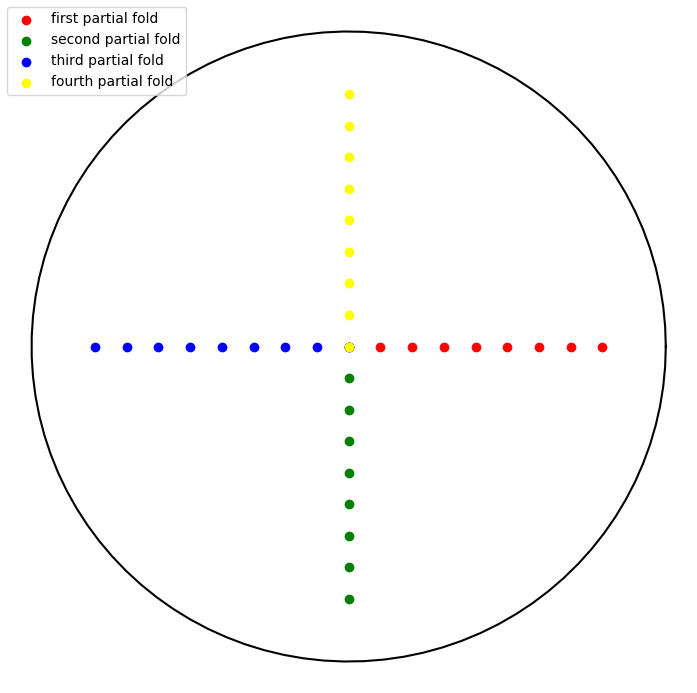
\includegraphics[scale=0.35]{Graphics/motions/folding0.png}
    \centering
    \label{fig:foldingMotion1}
    \caption{Top Down View - Folding 4 areas of a container}
\end{figure}

In this example the folding motion is applied onto four different areas of the circular container. 
It doesn't really matter how many areas are covered or at what angle the folding line is adjusted. 
The core movement remains the same: the motion is executed in a line and then returns.

Once the folding motion has been executed, to cover different parts of the container, we apply a transformation with a different angle $\phi$

\begin{figure}[H]
    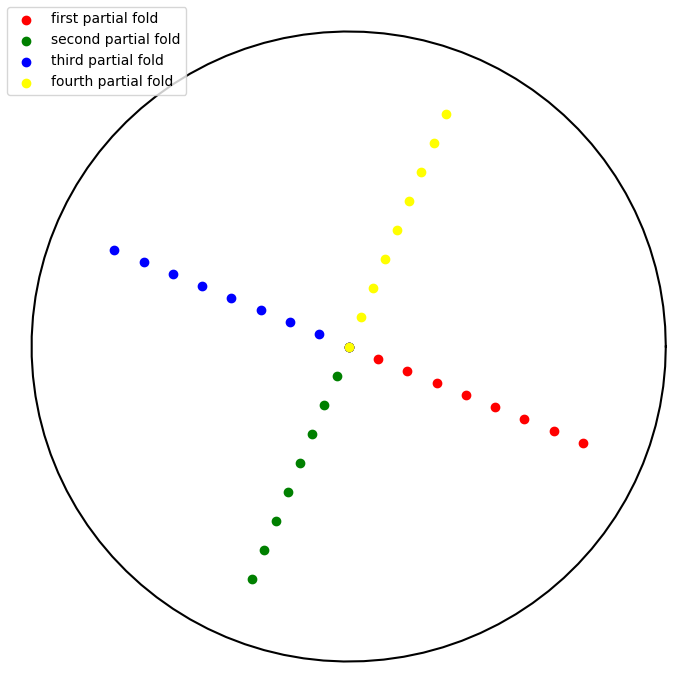
\includegraphics[scale=0.35]{Graphics/motions/folding1.png}
    \centering
    \label{fig:foldingMotion1}
    \caption{Cover different areas of the container}
\end{figure}

\section{Horizontal Elliptic Motion}
The horizontal elliptic motion is executed on a horizontal plane and involves multiple ellipses.
Using the function to compute x,y coordinates on a circle, we use two different radii.
One radius equals the radius of a given container, and the other radius is sampled from an interval. The interval is defined as \[radii = [radius, \frac{radius} {2} ]\]
meaning the sampled radius ranges from the full radius of the container to half of that radius.


A sampled radius from this interval is taken, if the following condition is true for all resulting circle coordinates:
\[\sqrt{(xCord - xCenter)^2 + (yCord - yCenter)^2} < radius\] 

To cover most areas of any container and assuming that generating y-coordinates used a constant radius, all y-coordinates are shifted after generating the ellipses. 
To check if the y-coordinates are within the container's bounds, the following condition is checked for every y-coordinate:

\[\sqrt{(yCord)^2 + (yCenter)^2} < radius\]

If this condition is met, the direction of the shift is reversed, switching from incrementing to decrementing and vice versa.

The horizontal elliptic motion can look like this:

\begin{figure}[H]
    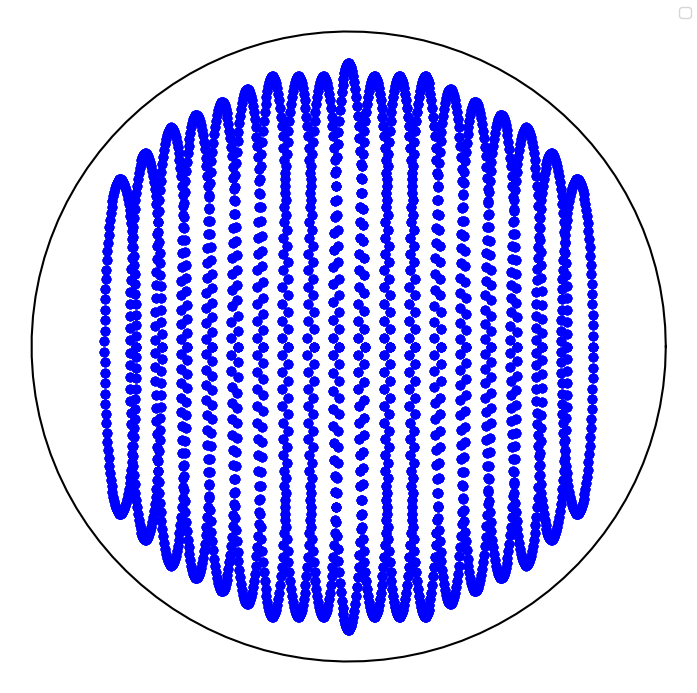
\includegraphics[scale=0.35]{Graphics/motions/horizontal_elliptical.png}
    \centering
    \label{fig:foldingMotion1}
    \caption{Multiple ellipses covering the containers area}
\end{figure}



\section{Whirlstorm Motion}
The whirlstorm motion uses the function to generate points lying inside a circle, with differing radiuses, over the course of the motion. 
Using an upper bound radius and a lower bound radius, we create an evenly spaced interval between those radiuses, to use them for coordinate generation. 
Starting from the upper bound to the lower bound translates to performing the motion from the edge to the center or close to the center, depending on the 
values of upper and lower bound radius. 

To create a consistent and fluid motion, we introduce mirroring of the coordinates and alternating from outer to inner circular motion and vice versa.
These are visualized in these plots:


